\documentclass[twocolumn]{article}
\usepackage{array,url,kantlipsum}
\usepackage{lmodern}
\usepackage{tikz}
\usepackage{capt-of}
\usepackage{biblatex}
\usepackage{graphicx}

\usetikzlibrary{arrows,decorations.pathmorphing}

\addbibresource{paperdyna.bib}

\tikzset{>=latex}

\tikzset{snake it/.style={decorate, decoration=snake}}

% \Mark is probably provided by spconf, that I don't have
\newcommand{\Mark}[1]{\textsuperscript{#1}}

\begin{document}
\twocolumn[{%
 \centering
 \LARGE Fuzzy ARIMA model vs naive model  \\[1.5em]
 \large Repetto Marco\Mark{1},
       \\[1em]
 \normalsize
 \begin{tabular}{*{2}{>{\centering}p{.35\textwidth}}}
  \Mark{1}Dipartimento di Management e Metodi Quantitativi \tabularnewline
  Università degli studi di Milano \tabularnewline
  \url{}marco.repetto@studenti.unimi.it
 \end{tabular}\\[3em] % some more space after the title part
}]

\begin{abstract}
This paper present the combination of an ARIMA process with the notion of fuzzy set. Such combination is used for signal generation in the prediction of stock prices, especially in such case the goodness of such model is tested in comparison with a naive algorithm. The portfolio of such game is built using common stocks from NASDAQ.
\end{abstract}

\section{Introduction}
Trading on securities is probably one of the many field in finance which saw an incredible automatization over recent years and consequently an improvement in efficiency in the markets interested in such innovation\cite{AvellanedaAlgorithmicHighfrequencytrading2011}.

\begin{figure}
    \centering
    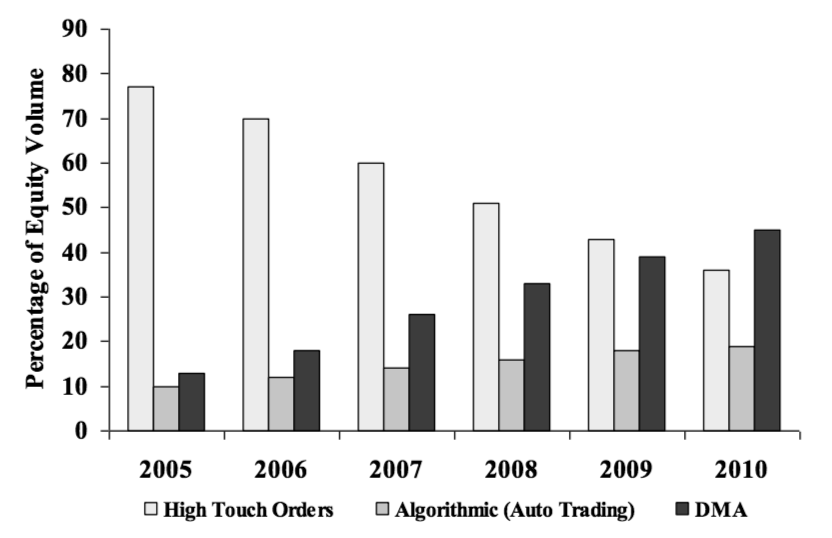
\includegraphics[width=1\linewidth, ]{images/algodata.png}
    \caption{Percentage of order generated by algorithms}
    \label{algodata}
\end{figure}

A completely new professional role came out from such innovation; the Quant, that is, a professional who is expert in quantitative analysis and in particular in financial modelling. The concept of Quant would not be so important without the concept of algorithmic trading, which is defined as automated trading done by computers which are programmed to take certain actions in response to varying market data. In very simplistic and kind of "naive" words the algorithm take the inputs from the model developed by the Quant and enacts the decision supported by the financial model.
In order to let the algorithm implement market decisions (whether to buy or to sell a particular security) we have to "feed" it with a proper financial model. A tipycal algorithmic trading process would is represented on figure \ref{algoproces}; the overall process consists mainly in 4 cyclical phases where two of them interacts comprehend interactions with the environment, as follows:

\begin{itemize}
\item I phase: consists manly on data gathering from the environment $E$, in our case since we are using an univariate time series model our data comes form the sub set $M$ which represent the market data;
\item II phase: at this point the data gathered are used by the quant to create a proper financial model able to forecast the behaviour of the securities under scope; 
\item III phase: this phase embrace the activities of backtesting of the financial model built by the professional;
\item V phase: eventually the financial moodel is deployed and starts to interact with the market $M$.
\end{itemize}


In this paper we decided to operate a forecast using a model based on time series, precisely an ARIMA (Auto Regressive Integrated Moving Average) process. Plus following what reported by Tseng et al.\cite{TsengFuzzyARIMAmodel2001} we associated to ARIMA process the fuzzy regression %mettere riferimento
and we defined an algorithm for pseudo real-time signal generation. Based on such signal the algorithm enact the decision whether to buy a stock (forecasting its increase in price) or sell it (because the price will fall). The overall model has to compete with a "naive" algorithm that perform buy and sell decision based only on the condition that the last price is major than the current one, and sell it when the such price raises.

\begin{center}
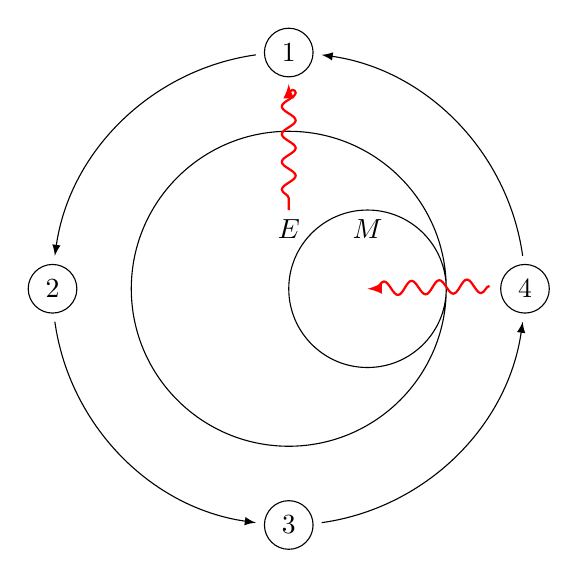
\begin{tikzpicture}

\def \n {4}
\def \radius {3cm}
\def \margin {8} % margin in angles, depends on the radius

  \node[draw, circle] at ({360/\n * (1 - 1)}:\radius) {$4$};
  \draw[->, >=latex] ({360/\n * (1 - 1)+\margin}:\radius) 
    arc ({360/\n * (1 - 1)+\margin}:{360/\n * (1)-\margin}:\radius);
    
     \node[draw, circle] at ({360/\n * (2 - 1)}:\radius) {$1$};
  \draw[->, >=latex] ({360/\n * (2 - 1)+\margin}:\radius) 
    arc ({360/\n * (2 - 1)+\margin}:{360/\n * (2)-\margin}:\radius);
    
     \node[draw, circle] at ({360/\n * (3 - 1)}:\radius) {$2$};
  \draw[->, >=latex] ({360/\n * (3 - 1)+\margin}:\radius) 
    arc ({360/\n * (3 - 1)+\margin}:{360/\n * (3)-\margin}:\radius);
    
     \node[draw, circle] at ({360/\n * (4 - 1)}:\radius) {$3$};
  \draw[->, >=latex] ({360/\n * (4 - 1)+\margin}:\radius) 
    arc ({360/\n * (4 - 1)+\margin}:{360/\n * (4)-\margin}:\radius);


\draw (0,0) circle (2) (0,1)  node [text=black,below] {$E$}
      (1,0) circle (1) (1,1)  node [text=black,below] {$M$};
\path [->, thick,draw=red,snake it]
    ({360/5 * (0.9 - 1)+\margin}:2.55) -- (1,0);
\path [<-, thick,draw=red,snake it]
    ({(360/\n * (2 - 1))}:2.6) -- (0,1);
%\draw[draw=blue, snake it] (2,0) arc (0:180:2cm);

\end{tikzpicture}
\end{center}
\captionof{figure}{Algorithmic trading process}
\label{algoproces}
\subsection{Auto Regressive Integrated Moving Average: key concepts and features}
ARIMA process are a class of univariate time series models, this kind of models attempt to predict financial variables using only information contained in their own past values and possibly current and past values of an error term.

\printbibliography

\end{document}